\chapter{Results}\label{Sec:Results}

\section{Maximal Representative Subsample}

There is almost always not enough data available to partition it into separate training and test sets without losing significant modelling or testing capability. In these cases, a fair way to properly estimate model prediction performance is to use cross-validation as a powerful general technique[5].

The overly optimistic resubstitution error, is not a good indicator of model performance. To evaluate the actual performance of a model, the given data samples need to be split. The proper procedure uses three sets: training data, validation data, and test data [2]. The holdout method is the most common approach to get a reliable performance estimation: A certain amount of data is reserved for testing while the remainder is used for the actual training. Because the method is very fast, it is useful to use when the algorithm is slow to train and the dataset is large. Training and test sets might not be representative of the same underlying distribution, e.g. class hardly represented in the test set.

\begin{table}[ht]
    \begin{center}
            {\footnotesize
            \begin{tabular}{l|cccccccccc}
                \hline \hline
                           &  TP Rate & FP Rate & Precision & Recall & F-Measure & ROC Area & PRC Area & Class \\
                \hline
                      & 0.000 & 0.000 & ? & 0.000 & ? & 0.500 & 0.130 & GBS &\\
                      & 1.000 & 1.000 & 0.870 & 1.000 & 0.931 & 0.500 & 0.870 & GESIS &\\
                \hline \hline
		 W. Avg. & 0.870 & 0.870 & ? & 0.870 & ? & ? & 0.500 & 0.774 &
            \end{tabular}}
        \caption{Some descriptive statistics of location and dispersion for 2100 observed swap rates for the period from February 15, 1999 to March 2, 2007. Swap rates measured as 3.12 (instead of 0.0312). See Table \ref{Tab:DescripStatsRawDataDetail} in the appendix for more details.}
\label{Tab:DescripStatsRawData}
\end{center}
\end{table}

The holdout estimate can be made more reliable by repeating the process with different subsamples. The error rates on the different iterations are averaged to yield an overall error rate. To further reduce the variance of the error estimate, each class is sampled with approximately equal proportions in both datasets, a technique called stratification. Figure X shows the results on the GFI-10 data.

Estimating positive class prior with One-Class SVMs.

\begin{figure}[ht]
	\begin{center}
		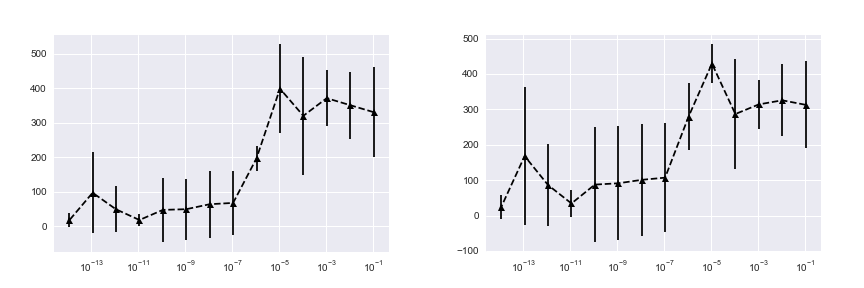
\includegraphics[scale=0.50,angle=0]{fig/occfigure}
		\label{occ}
		\caption{Using the One-Class SVM and its ability to capture the fraction of positive. Tuning parameter \(nu\) that controls the trade-off between the fraction of non-representative samples and the number of support vectors in one-class SVM. More than 0.73 of GBS (right) are classified as representative with high confidence (low sdt) for the optimal value \(nu = 10^{-5}\).}
	\end{center}
\end{figure}

\begin{figure}[ht]
\centering
   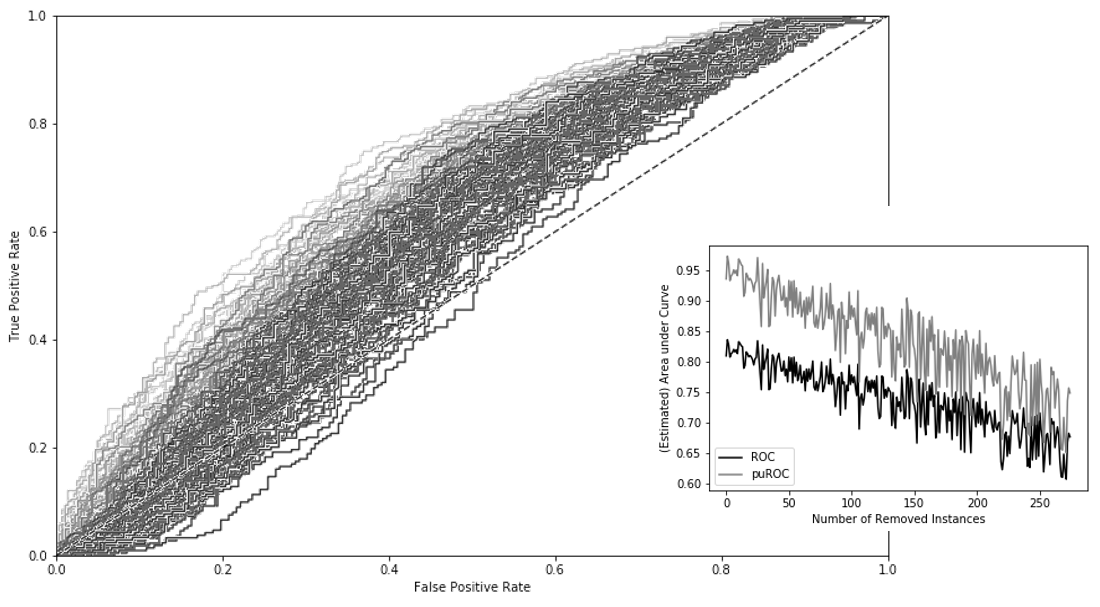
\includegraphics[scale=0.50,angle=0]{fig/res1}
\caption{ROC and puROC Evaluation.}
   \label{fig:Ng1} 
\end{figure}

\begin{figure}[ht]
\centering
\begin{subfigure}[b]{0.8\textwidth}
   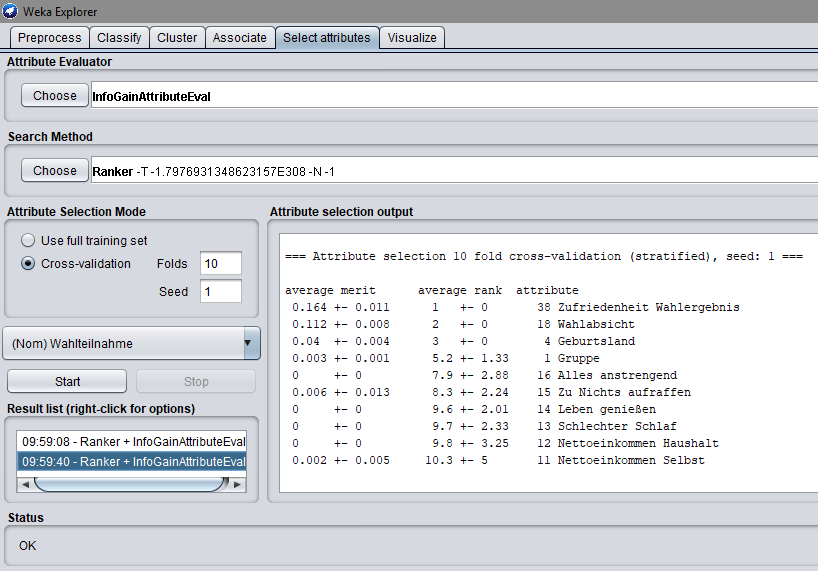
\includegraphics[scale=0.55,angle=0]{fig/weka_gbs}
   \label{fig:Ng1} 
\end{subfigure}
\begin{subfigure}[b]{0.8\textwidth}
\vspace{0.55cm}
   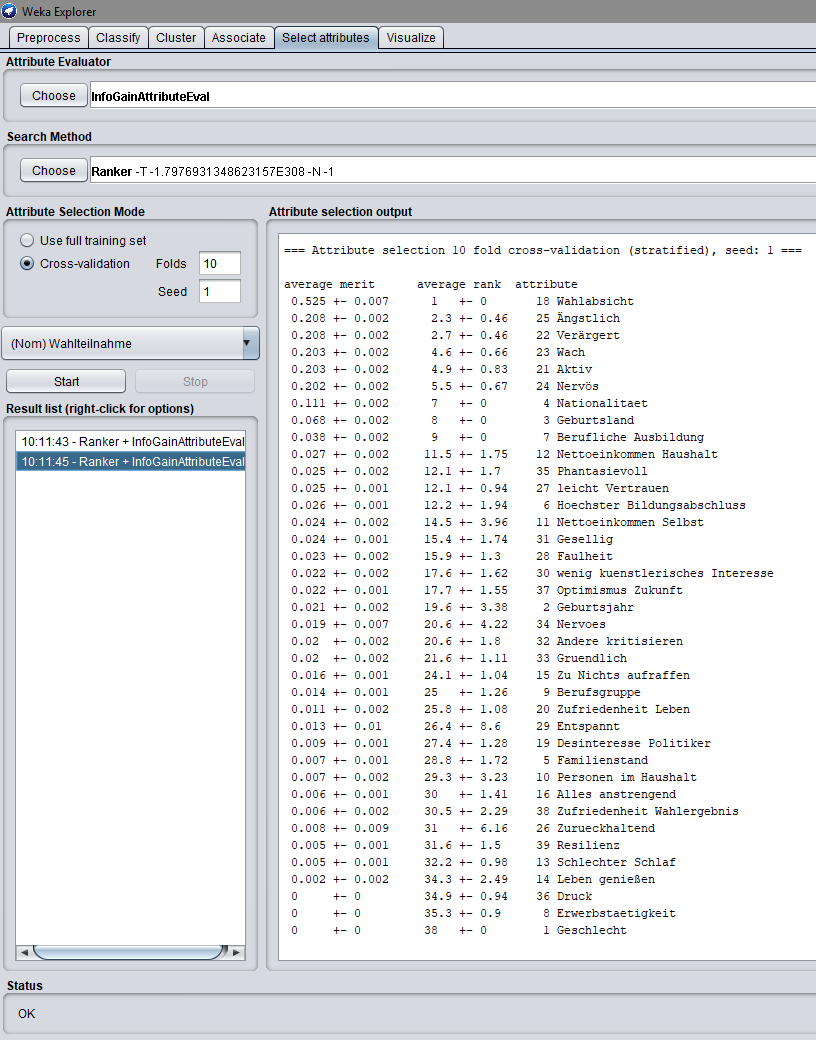
\includegraphics[scale=0.55,angle=0]{fig/weka_gesis}
   \label{fig:Ng2}
\end{subfigure}
\vspace{0.35cm}
\caption{Feature importance in GBS (n=579) and GBS MRS (n=280) for classification of political participation "Wahlteilnahme". In modelling a political participation process, algorithms approximate the likelihood of a person going to vote on election day. Ideally, for every instance with unknown political interest and willingness to participate, there is enough data of people of similiar demographics, socioeconomics and psychological traits to generalize from.}
\end{figure}

\section{Future Work}

Many different adaptations, statistics, and experiments have been left for the future due to lack of time, i.e. data matching and transformation with real data have been very time consuming. Controlled environments are needed to observe the behavior of the proposed algorithm.

For one thing, future work concerns deeper analysis of the proposed sampling method, in particular, experiments on synthezised data. The Synthetic Minority Over-sampling TEchnique (SMOTE \cite{smote}) is a very popular oversampling method that creates synthetic minority class instances. The SMOTE instances are linear combinations of two similar instances from the minority class (\(x\) and \(x^{R}\)) and are defined as: \(s = x + u (x^{R} - x) \) with \(0 \geq  u \geq 1\). \(x^{R}\) is randomly chosen among the \(k\) nearest neighbors of \(x\) belonging to the minority class. SMOTE can be used to validate the MRS procedure by simulating the problem at hand.

Specific regions in the feature space are first over-sampled using SMOTE, before they are under-sampled by MRS. Experiments with multiple such synthesized data, with oversampling ratio ranging from high to low, might support the proposed procedure with greater evidence. The initial data sets are then compared to the result sets. GESIS is particularly well suited to artificially recreate the initial problem as visualized in Figure 5.1. It is only necessary to try to avoid giving the synthesized data properties that makes it possible for a learning algorithm to distinguish synthesized from non-synthesized example. This mechanism would for instance aid to compare classification results more easily.

\begin{figure}[ht]
	\begin{center}
\vspace{0.5cm}
		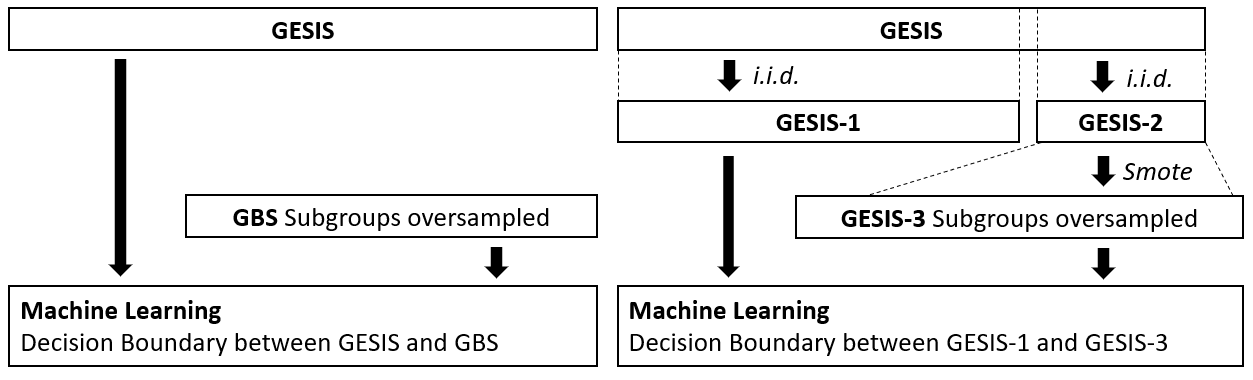
\includegraphics[scale=0.41,angle=0]{fig/procedure2}
		\label{std}
		\caption{Artificial data synthesis to overrepresent subgroups of GESIS. True negatives are removed from the MRS with positive classes GESIS (left) and GESIS-1 (right). Oversampled instances can easily be marked as such for result set comparisons.}
	\end{center}
\end{figure}

The main criteria considered in this work has been the area under the ROC curve. Having a single-number evaluation metric speeds decision-making when selecting among non-representative instances. It gives a clear preference ranking among all of them, and therefore a clear direction for progress. To enable a basis for a more informed exclusion of instances, another important performance criterion generally used in information retrieval could be added. The F-Measure, including summary statistics derived from the precision-recall curve, may be preferred to ROC curves when classes are heavily skewed \cite{jesse}. Precision and recall have been estimated in section 3.3.1 in a positive-unlabeled setting. The area under precision-recall curves \(AUPR\) can be expressed using the approximated value for the fraction of positives \(\alpha\) in \(X_u\): \(\rho = \frac{\alpha \gamma}{\hat{\eta}^{pu}}\).

